\documentclass[11pt]{article}
\usepackage[utf8]{inputenc}
\usepackage[T1]{fontenc}
\usepackage{amsmath,amssymb}
\usepackage{geometry}
\usepackage{listings}
\usepackage{xcolor}
\usepackage{hyperref}
\usepackage{tikz}
\usepackage{booktabs}
\usetikzlibrary{calc, arrows.meta, positioning, decorations.pathmorphing}

\geometry{margin=2.5cm}

\lstdefinelanguage{Rust}{
  keywords={fn,let,mut,for,in,if,else,while,loop,match,return,struct,impl,pub,use,mod,as,where,move,ref,self,Self,crate,super,async,await,unsafe,const,static,type,enum,trait, dyn, true, false, continue, break},
  keywordstyle=\color{blue!70!black}\bfseries,
  ndkeywords={Vec,Vec3,Mat4,Mesh,MeshVertex,SceneNode,Scene,PbrMaterial,Affine3A,u32,usize,f32,f64,bool,Option,Some,None,Result,Ok,Err,String},
  ndkeywordstyle=\color{purple!70!black}\bfseries,
  sensitive=true,
  comment=[l]{//},
  morecomment=[s]{/*}{*/},
  commentstyle=\color{green!50!black}\itshape,
  stringstyle=\color{red!70!black},
  morestring=[b]",
}

\lstdefinelanguage{wgsl}{
  keywords={fn,let,var,if,else,for,while,loop,return,struct,uniform,storage,binding,group,vertex,fragment, true, false},
  keywordstyle=\color{blue!70!black}\bfseries,
  ndkeywords={vec3,vec4,mat3x3,mat4x4,f32,u32,bool,normalize,dot,max,clamp,reflect,mix},
  ndkeywordstyle=\color{purple!70!black}\bfseries,
  sensitive=true,
  comment=[l]{//},
  commentstyle=\color{green!50!black}\itshape,
  stringstyle=\color{red!70!black},
  morestring=[b]",
}

\lstset{
  basicstyle=\ttfamily\footnotesize,
  breaklines=true,
  frame=single,
  language=Rust,
  showstringspaces=false,
  tabsize=2,
}

\title{Gyroid-Sphere: Open-Surface Construction by\\
       Spherical Clipping, with a Two-Sided Lighting Pitfall}
\author{engvis}
\date{\today}

\begin{document}
\maketitle

\section{Goal}

Render the gyroid implicit surface
\[
  f(x,y,z)=\sin x\cos y+\sin y\cos z+\sin z\cos x \;=\; 0
\]
\emph{restricted to the open ball} $B = \{\mathbf{p}:\|\mathbf{p}\|<R\}$
with $R = 1$.  The result is a single open surface patch
\[
  S \;=\; \{f = 0\} \cap B,
\]
not a closed solid: only the gyroid two-manifold inside the ball, with
its boundary lying exactly on the sphere $\partial B$.

\section{Why Boolean SDF Combinations Are Wrong}

A first instinct is to combine the gyroid SDF $g$ and the ball SDF
$s = \|\mathbf{p}\| - R$ with a Boolean op:

\begin{table}[h]
  \centering
  \begin{tabular}{lll}
    \toprule
    Operator & Set produced & What we get \\
    \midrule
    $\min(g,s)$ & union  & gyroid + ball envelope \\
    $\max(g,s)$ & intersection & gyroid ``capped'' by ball faces \\
    \bottomrule
  \end{tabular}
\end{table}

Both produce a \emph{closed solid} (gyroid skin plus a spherical cap),
not a thin two-manifold.  This is the wrong topology: the iso-surface
$\{g=0, s\le 0\}$ is a 2-manifold with boundary, while
$\{\max(g,s)=0\}$ is the boundary of a 3-manifold and contains spurious
``cap'' regions where $g>0$.

\section{Construction: Pure Gyroid Mesh + Spherical Mesh Clipping}

The chosen pipeline (Figure~\ref{fig:pipeline}) keeps $g$ pure and clips
the resulting triangle mesh:

\begin{figure}[h]
  \centering
  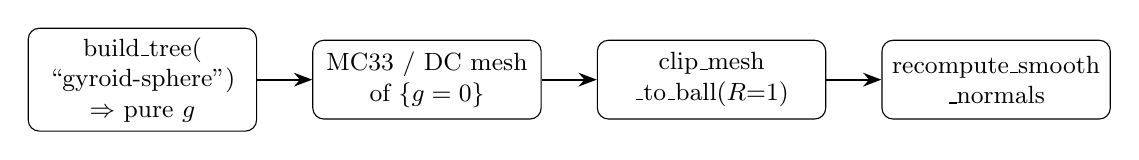
\begin{tikzpicture}[
      node distance=6mm and 7mm,
      box/.style={draw, rounded corners, align=center, minimum height=10mm,
                  minimum width=29mm, font=\small},
      arr/.style={-Stealth, thick}
    ]
    \node[box] (tree) {build\_tree(\\``gyroid-sphere'')\\$\Rightarrow$ pure $g$};
    \node[box, right=of tree] (mc) {MC33 / DC mesh\\of $\{g=0\}$};
    \node[box, right=of mc] (clip) {clip\_mesh\\\_to\_ball($R{=}1$)};
    \node[box, right=of clip] (norm) {recompute\_smooth\\\_normals};

    \draw[arr] (tree) -- (mc);
    \draw[arr] (mc)   -- (clip);
    \draw[arr] (clip) -- (norm);
  \end{tikzpicture}
  \caption{\label{fig:pipeline} gyroid-sphere construction.  The implicit
    tree is the pure gyroid; the ball is enforced as a post-processing
    step on the triangle mesh.}
\end{figure}

\subsection{Exact spherical cutting}

For each triangle $(V_0,V_1,V_2)$ let $d_i = \|V_i-c\|^2 - R^2$.  An
inside vertex satisfies $d_i\le 0$.  We classify the triangle by the
number $k$ of inside vertices:

\begin{itemize}
  \item $k=3$: keep verbatim.
  \item $k=0$: discard.
  \item $k=1$: split into one new triangle $(V_\text{in},A,B)$ where
        $A,B$ are the sphere-edge intersections.
  \item $k=2$: split into two triangles
        $(V_\text{next},V_\text{prev},A)$ and
        $(V_\text{next},A,B)$ to fill the remaining quad.
\end{itemize}

The intersection on edge $(V_a,V_b)$ is solved analytically.  Writing
$P(t) = V_a + t(V_b-V_a)$ and substituting into
$\|P-c\|^2 = R^2$ gives a quadratic; the inside--outside transition
gives the linear approximation
\[
  t \approx \frac{d_a}{d_a - d_b},
\]
which is sufficient since $|d_a|+|d_b|$ is small relative to $R^2$ at
mesh resolution.  The resulting boundary vertices lie on $\partial B$
to numerical precision.

\subsection{Why we recompute smooth normals after clipping}

The clip introduces new vertices with zero normals.  We initially tried
to overwrite all normals using the analytic gradient $\nabla g$ via
\texttt{overwrite\_normals\_with\_gradient}.  Empirically the
\texttt{fidget} grad evaluator returned $(0,0,0)$ for these points; the
function silently keeps the old normal.  For untouched gyroid vertices
this was harmless because \texttt{from\_triangles\_open} had already
filled in smooth normals.  For the new clip vertices it left the
normals at zero --- causing the ``black surface'' bug
(Section~\ref{sec:black}).

The fix is the standalone helper
\texttt{recompute\_smooth\_normals(\&mut mesh)}, which computes
area-weighted vertex normals from triangle geometry alone:
\[
  \mathbf{n}_v
  \;=\;
  \frac{
    \displaystyle\sum_{T \ni v}\bigl(\mathbf{p}_1-\mathbf{p}_0\bigr)\times
                                  \bigl(\mathbf{p}_2-\mathbf{p}_0\bigr)
  }{
    \bigl\|\,\sum_T (\cdots)\,\bigr\|
  }.
\]
This depends only on the mesh and so works after the clip.

\section{Black-Surface Bug, Three Layers Deep}\label{sec:black}

After the clip pipeline was complete, the gyroid-sphere patch rendered
\emph{very dark}, while gyroid (no clip) looked correct.  Three
distinct issues conspired:

\subsection{Layer 1: Open back face never lit}

After the clip the mesh is open: the back side of the gyroid sheet now
faces the camera at oblique angles.  Standard back-face culling
(\texttt{cullMode = Back}) drops half the triangles.  We turned off
back-face culling, but with $\cos\theta = \mathbf{N}\cdot\mathbf{L}$
clamped to $\ge 0$, the back-facing fragments returned $\cos\theta=0$
and thus zero diffuse, leaving them lit only by ambient.

The standard remedy is two-sided lighting: in the fragment shader, if
the geometric normal faces away from the camera, flip it.

\begin{lstlisting}[language=wgsl]
let V = normalize(scene.camera_pos - in.world_position);
if (dot(N, V) < 0.0) { N = -N; }
\end{lstlisting}

\subsection{Layer 2: NaN propagation from a zero tangent}

Even after enabling two-sided lighting, the patch was still very dark.
Inspection of one fragment showed
$L_\text{out} \approx \texttt{ambient}$, exactly as if
$\cos\theta\equiv 0$.

The root cause was the \emph{tangent}, not the normal.  Newly created
clip vertices were initialised with
\texttt{tangent = [0.0, 0.0, 0.0, 1.0]}.  The shader does

\begin{lstlisting}[language=wgsl]
let T = normalize(in.world_tangent);  // normalize([0,0,0]) = NaN
let TBN = mat3x3<f32>(T, B, Ng);
var N = normalize(TBN * sampled_normal);
\end{lstlisting}

\(\texttt{normalize}([0,0,0])\) is NaN; the TBN matrix is poisoned;
\(N\) is NaN; \(\max(\mathbf{N}\cdot\mathbf{L},0)=0\) drops the entire
diffuse and specular term.  Fix: set the new vertices' tangent to
\([1,0,0,1]\), matching what \texttt{from\_triangles\_open} writes for
its own vertices.

\subsection{Layer 3: Zero normals, masked by a gradient overwrite}

A second invisible factor was that \emph{all} clip-vertex normals were
$[0,0,0]$.  We thought
\texttt{overwrite\_normals\_with\_gradient} repaired them, but the
fidget grad evaluator returned zero gradients for every point we
tried; the function's
\texttt{if len > 1e-10} guard then skipped the overwrite, leaving the
zeros in place.  For the original gyroid mesh this was masked by the
prior smooth-normal pass.  For clip vertices it was not.

The two-line fix was to call \texttt{recompute\_smooth\_normals(\&mut
mesh)} \emph{after} the clip --- a pure mesh-geometry computation that
cannot fail in this way.

\subsection{Pipeline of the fix}

\begin{figure}[h]
  \centering
  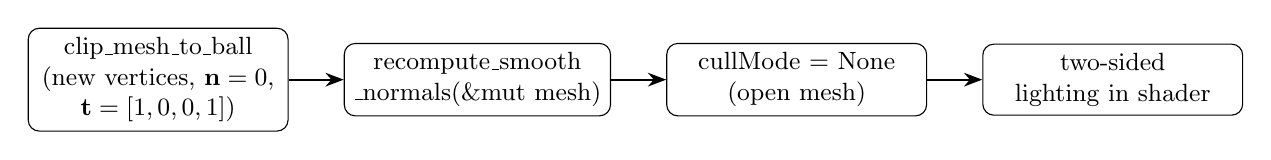
\begin{tikzpicture}[
      node distance=5mm and 7mm,
      box/.style={draw, rounded corners, align=center, minimum height=9mm,
                  minimum width=33mm, font=\small},
      arr/.style={-Stealth, thick}
    ]
    \node[box] (clip)   {clip\_mesh\_to\_ball\\(new vertices, $\mathbf{n}=0$,\\$\mathbf{t}=[1,0,0,1]$)};
    \node[box, right=of clip] (sn)
      {recompute\_smooth\\\_normals(\&mut mesh)};
    \node[box, right=of sn] (cull)
      {cullMode = None\\(open mesh)};
    \node[box, right=of cull] (ts)
      {two-sided\\lighting in shader};

    \draw[arr] (clip) -- (sn);
    \draw[arr] (sn)   -- (cull);
    \draw[arr] (cull) -- (ts);
  \end{tikzpicture}
  \caption{\label{fig:fix} Four pieces had to align for the clipped
    patch to be lit correctly: non-zero tangents, geometry-based
    normals, no back-face culling, and two-sided lighting.  Removing
    any one yields a dark mesh.}
\end{figure}

\section{Lessons Learned}

\begin{itemize}
  \item For open implicit-surface patches, prefer \emph{mesh-level}
        clipping over Boolean SDF combinations.  The latter changes
        topology from 2-manifold to 3-manifold boundary and introduces
        spurious cap regions.
  \item Never rely on a numerical gradient as the sole source of
        vertex normals: a silent zero-gradient evaluation degrades to
        ``no normals'' rather than an error.
  \item Watch for NaN-propagation paths through \texttt{normalize(...)}
        --- a single zero-length vector
        in a TBN frame can blacken every fragment using that vertex.
  \item Two-sided lighting (back-normal flip) is the default for any
        open mesh whose triangles can present either face to the
        camera.
\end{itemize}

\section{Implementation Pointers}

\begin{itemize}
  \item \texttt{src/main.rs}
        \begin{itemize}
          \item \texttt{clip\_mesh\_to\_ball(mesh, c, r)} --- exact
                spherical cutting of triangles.
          \item \texttt{recompute\_smooth\_normals(\&mut mesh)} ---
                area-weighted normals from triangle geometry alone.
          \item In \texttt{build\_mesh}: after MC33/DC and the clip,
                call \texttt{recompute\_smooth\_normals}.
          \item Clip-vertex initialiser uses
                \texttt{tangent = [1.0, 0.0, 0.0, 1.0]}.
        \end{itemize}
  \item \texttt{crates/engvis-renderer/src/material\_pipeline.rs}
        \begin{itemize}
          \item Solid pipeline: \texttt{cullMode = None}.
          \item Fragment shader: \texttt{if dot(N,V) < 0.0 \{ N = -N; \}}
                before lighting.
        \end{itemize}
\end{itemize}

\end{document}
